\documentclass[11pt]{beamer}

% language specific settings
\usepackage[english]{babel}
\usepackage[utf8x]{inputenc}

% packages
\usepackage{graphicx}
\usepackage{url}
\usepackage{booktabs}
\usepackage[numbers,sort&compress]{natbib}
\bibliographystyle{plainnat}

% images path
\graphicspath{{images}{../images}}

\mode<presentation>
{
    \usetheme[progressbar=frametitle]{metropolis}
    \usefonttheme{serif} 
    \setbeamertemplate{navigation symbols}{}
    \setbeamertemplate{caption}[numbered]
} 

\title{Object detection with TensorFlow}
\date{03/28/2019}
\author{Caglar Özel}
\institute{HTW Berlin}

\begin{document}

\begin{frame}
    \titlepage
\end{frame}

\begin{frame}{Table of Content}
    \tableofcontents
\end{frame}

\section{Introduction}
\begin{frame}{What is computer vision?}
    \begin{itemize}
        \item Images are a bunch of colored dots (pixels)
        \item Videos and Streams are a bunch of images in a loop
        \begin{figure}
            \begin{center}
                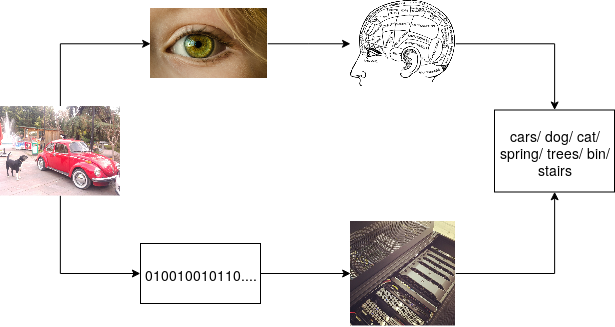
\includegraphics[width=0.75\textwidth]{images/Recoginition_Process.png}\cite{eye, brain, server}
            \end{center}
        \end{figure}
        \item Easily understood by the brain, impossible for the computer 
    \end{itemize}
\end{frame}

\begin{frame}{What is object detection?}
    \begin{itemize}
        \item Computer Vision: what is an image about \\
            (general topic / content)
        \begin{itemize}
            \item Object classification
        \end{itemize}
        \item Object Detection: where are the objects\\
            (content + location)
        \begin{itemize}
            \item Object localization \& Object classification
        \end{itemize}
    \end{itemize}
    \begin{figure}
        \begin{center}
            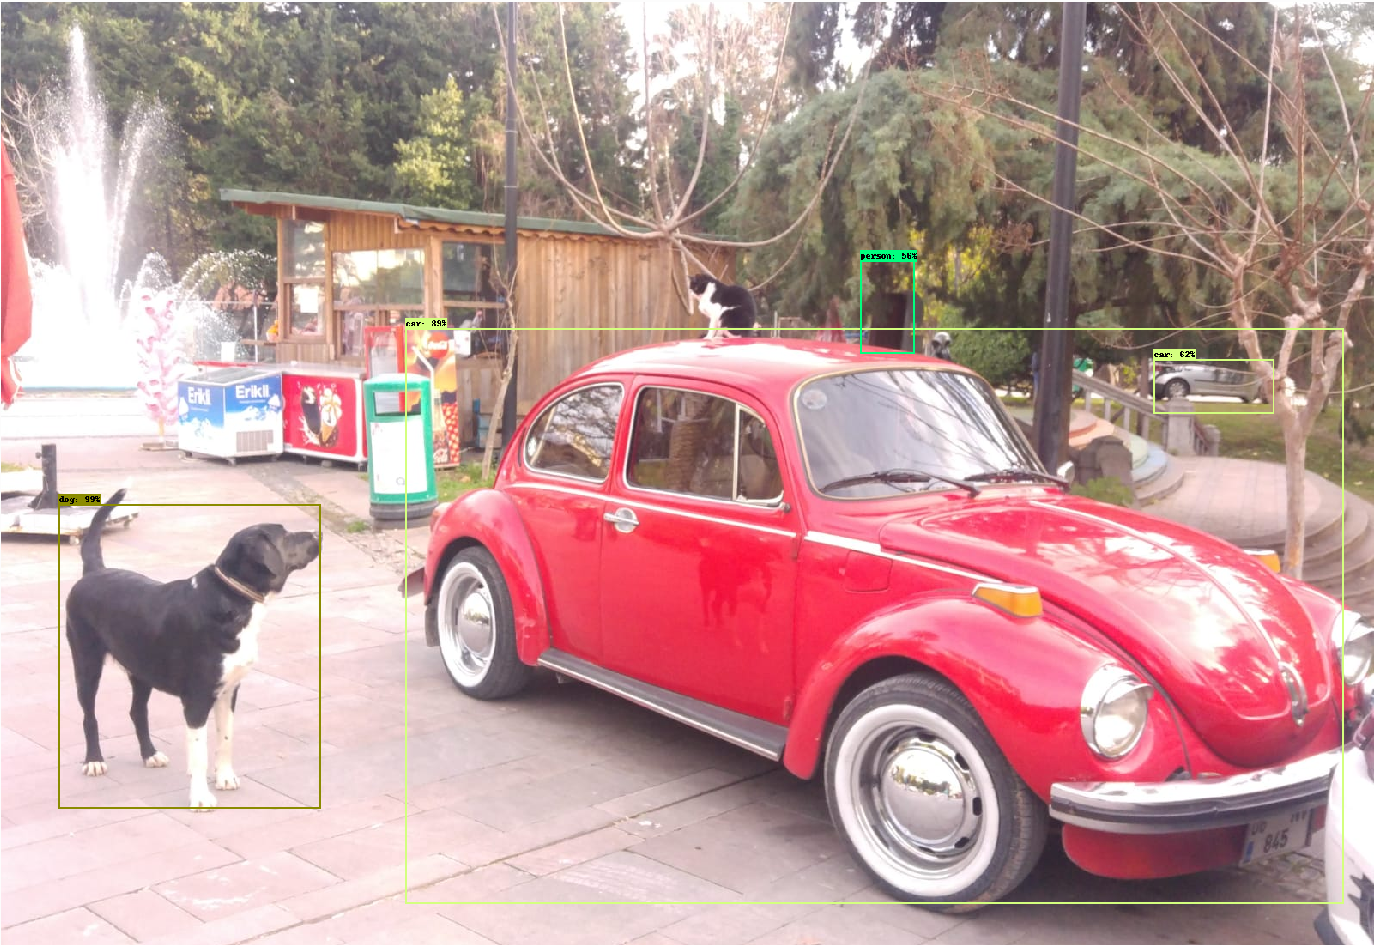
\includegraphics[width=0.7\textwidth]{images/Image_ObjectDetection.png}
        \end{center}
    \end{figure}
\end{frame}

\begin{frame}{Common problems in object detection}
    \begin{itemize}
        \item Unknown number of objects
            \begin{itemize}
                \item Requires post-processing to compensate
                \item Adds complexity to model
            \end{itemize}
        \item Scale, View point, Illumination, Occlusion
            \begin{itemize}
                \item Same objects may vary in size
                \item Object shape may change according to view point
                \item Object may look different under lighting
                \item May be covered by other objects
            \end{itemize}
        \item Modeling
            \begin{itemize}
                \item Concept of the model
                \item Perform multiple tasks
                    \begin{itemize}
                        \item in one layer vs multiple layers
                    \end{itemize}
            \end{itemize}
    \end{itemize}
\end{frame}

\begin{frame}{Current object detection models}
    \begin{itemize}
        \item R-CNN
        \item Faster R-CNN
        \item Yolo 
        \item SSD 
        \item R-FCN
    \end{itemize}
\end{frame}


\section{TensorFlow}
\begin{frame}{TensorFlow}

\end{frame}

\begin{frame}{Data model of TensorFlow}
    \begin{itemize}
        \item Training results per session stored in Checkpoints
        \item Results can be consulted on Tensorboard
    \end{itemize}
\end{frame}



\section{Application}
\begin{frame}{Application workflow}
\end{frame}


\begin{frame}{Resources}
    \bibliography{resources}
\end{frame}
\end{document}
